\label{sec:07Testofourmodels}
\section{Test of our models \& results}

\subsection{Models comparison} 
AIC and BIC values have been calculated with models of the de-seasonal de-trend time series. \\
For MAPE and RMSE values over the training period, we have recomposed the time series adding back the seasonal and trend components to the models. \\
For MAPE and RMSE values over the testing period, we had to recomposed the times series adding the forecast of both the seasonal and the trend component. A naive forecast is simple and efficient enough for the seasonal component. For the trend component, we have used several methods to forecast such as naive, arima, Holt-Winters, deterministic and stochastic regression.
\\
\underline{Remark :} A deterministic trend is obtained using the regression model $yt=\beta_0+\beta_1t+\eta_t$, where $\eta_t$ is an ARMA process. A stochastic trend is obtained using the model $yt=\beta_0+\beta_1t+\eta_t$, where $\eta_t$ is an ARIMA process with $d=1$.
\\
Tests performed have shown that a deterministic trend gives better results for ARMA models selected, stochastic trend is better for the ARIMA(5,1,0) model, Holt-Winters’ damped method is more appropriate for the SARIMA(5,1,0)(0,1,0). Thus we stored MAPE and RMSE values in the Table 11 for these combinations of models.
\\
\FloatBarrier
\begin{table}[!htbp]
  \centering
  \begin{tabular}{|l||*{10}{c|}}\hline
\backslashbox{Models}{Criteria}
&\makebox[3em]{AIC}&\makebox[3em]{BIC}&\makebox[5em]{MAPE(train)}
&\makebox[5em]{MAPE(test)}&\makebox[5em]{RMSE(train)}&\makebox[5em]{RMSE(test)}\\
\hline\hline
ARMA(1,0) &-7956.06&\textbf{-7940.59} & 0.000986549 &0.00404638& 0.0107792 &0.0422841\\\hline
ARMA(3,2) &-7961.87&-7925.79& 0.000982784 &0.00407286& 0.0107209 &0.0426170\\\hline
ARMA(7,7) &\textbf{-7979.10}&-7896.62& \textbf{0.000966084} &0.0040794&\textbf{ 0.0105547} &0.0427542 \\\hline
ARIMA(5,1,0)  &-7948.59&-7917.67& 0.000985010 &\textbf{ 0.00352064 } &0.0107656& \textbf{0.0362347} \\\hline
SARIMA(5,1,0)(0,1,0)  &-5466.16& -5436.58 & 0.00121570 &0.00463794&0.0148152&0.0486916\\\hline
H2O Deep Learning  &4400.623& N.A. & N.A. &0.02983843&N.A.&187.0266\\\hline
\end{tabular}
\caption{Models comparison}
\end{table}
\FloatBarrier

As wee can see in the Table 11 (where best value of each column is printed in bold), the ARMA(7,7) model has the best AIC, and so without surprise fit the best over the training period. However, over the testing period, this is the ARIMA(5,1,0) model which has the best MAPE and RMSE. We can also notice that ARMA(1,0), thanks to its lower numbers of parameters, has the best BIC values.



\subsection{Forecast}

According to the previous results, we chose  to look at forecasts from both ARMA(7,7) and ARIMA(5,1,0) models, as Figure 24 shows. \\

\FloatBarrier
\begin{figure}[!htbp]
  \centering
      \includegraphics[width=\textwidth]{img/FC.eps}
  \caption{Price forecast with ARMA(7,7) \& ARIMA(5,1,0)}
\end{figure}
\FloatBarrier

As we can see, both models predict a small drop in the price starting in May 2018, but an increase in the price over time. ARMA model is forecasting a higher price and a faster increase than ARIMA model, which makes us think that price in 2020 could approach the same values as ones in 2007 before the global crisis. However, it exists a significant gap between the first values predicted by the ARMA model and last values observed, so we could think that the model has kind of over-estimating issues.  
\\
We can conclude that price will probably suffer from a small drop, before increasing again. Since the ARMA model has had better performance over data out of the training sample, we can expect that the price will increase the same way it does in ARMA's prediction, but with lower values due to the starting gap of the prediction.

